\chapter{STUDI LITERATUR}
Untuk mendukung penelitian ini, telah dilakukan studi literatur terkait topik penelitian. Penelitian terkait tersebut direpresentasikan dalam peta literatur Gambar \ref{fig:literature-map}

\begin{figure}[H]
    \centering
    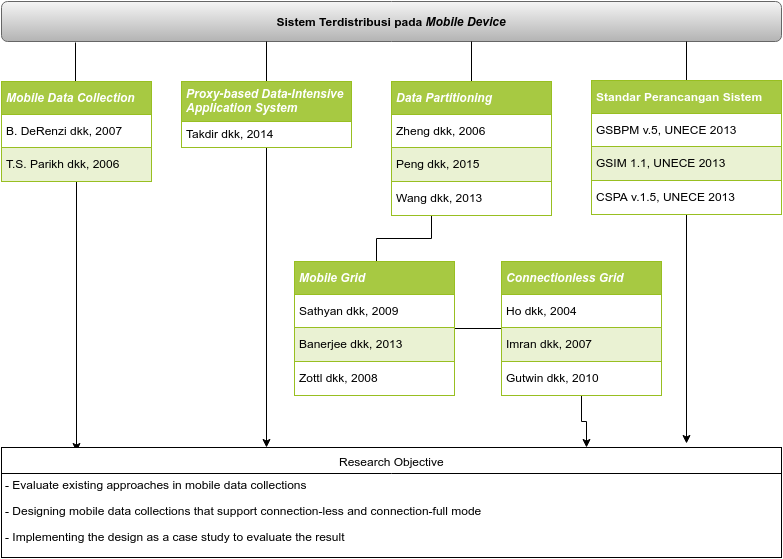
\includegraphics[height=6cm]{images/literature-map}
    \caption{\textit{Literature Map}}
    \label{fig:literature-map}
\end{figure}

\section{\textit{Generic Statistical Business Process Model (GSBPM)}}
GSBPM ~\cite{_gsbpm_????} mendefinisikan sekumpulan bisnis proses yang dibutuhkan untuk untuk kegiatan perstatistikan. GSBPM ditujukan untuk membantu institusi perstatistikan di dunia melakukan modernisasi pada kegiatan perstatistikan yang dijalankan. BPS juga telah mencanangkan untuk mengikuti bisnis proses pada GSBPM melalui program \textit{Statistical Capacity Building-Change and Reform for the Development of Statistics (STATCAP-CERDAS)}

\begin{figure}[H]
    \centering
    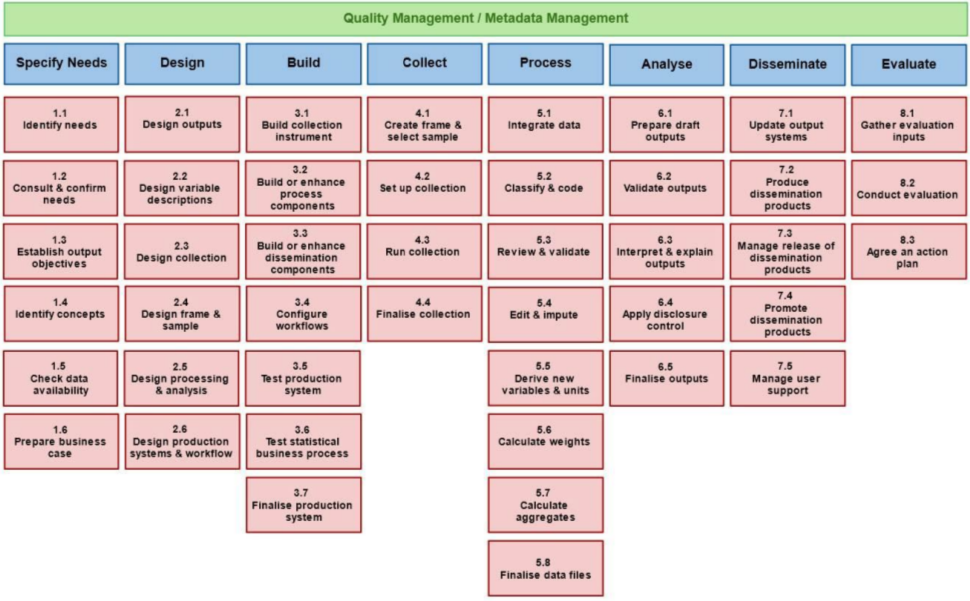
\includegraphics[height=5cm]{images/GSBPM}
    \caption{\textit{Statistical Business Process Phases} dalam GSBPM}
    \label{fig:gsbpm2}
\end{figure}

\section{\textit{Generic Statistical Information Model (GSIM)}}
GSIM merupakan \textit{framework model} informasi statistik internasional pertama yang diciptakan. GSBPM merupakan \textit{reference framework} untuk \text{information objects} pada kegiatan perstatistikan yang mendefinisikan penjelasan, pengelolaan dan penggunaan data dan metadata~\cite{_gsim_????}. GSIM dibentuk untuk memenuhi kebutuhan informasi pada proses-proses yang ada pada GSBPM. Pada level atas, GSIM mengelompokkan objek informasi menjadi 4 kategori, yakni \textit{Business}, \textit{Exchange}, \textit{Concepts}, dan \textit{Structures}.

\begin{figure}[H]
    \centering
    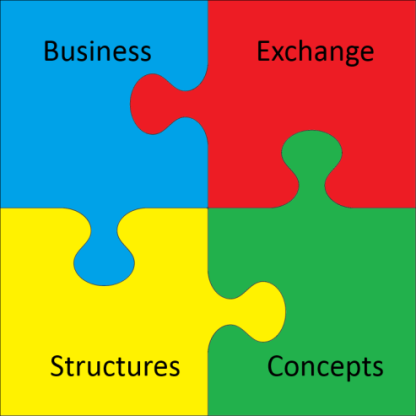
\includegraphics[height=4cm]{images/gsim}
    \caption{Kategori Objek pada GSIM}
    \label{fig:gsim}
\end{figure}

Selain itu, GSIM juga telah menetapkan spesifikasi teknis struktur data untuk tiap-tiap objek. Terdapat sebanyak 114 entitas yang telah didefinisikan oleh GSIM.

\begin{figure}[H]
    \centering
    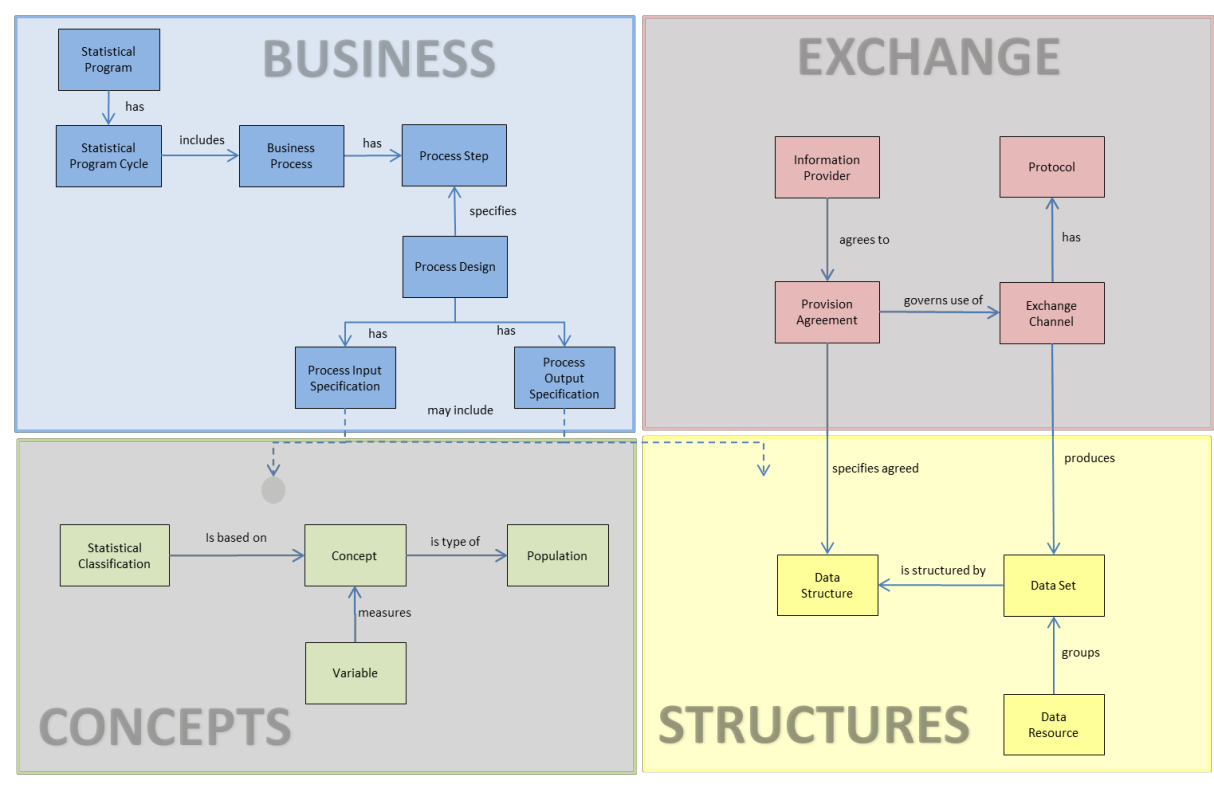
\includegraphics[height=5cm]{images/object-relation-gsim}
    \caption{Gambaran Sederhana Relasi Objek pada GSIM}
    \label{fig:object-relation-gsim}
\end{figure}

\section{\textit{Common Statistical Production Architecture (CSPA)}}
CSPA merujuk pada GSBPM sebagai arsitektur bisnis, GSIM sebagai arsitektur informasi, serta menggunakan pendekatan SOA (\textit{Service Oriented Architecture}) untuk arsitektur aplikasi dan arsitektur teknologi. Saat ini CSPA merupakan \textit{project} yang sedang aktif di UNECE. Project CSPA merupakan kolaborasi antara beberapa wakil di bidang TIK organisasi penyelenggara kegiatan perstatistikan dari berbagai negara guna merancang SOA untuk sistem perstatistikan~\cite{_cspa_????}. Tahap awal pada CSPA adalah mengidentifikasi kandidat layanan statistik (\textit{statistical services}). Hingga saat ini, CSPA telah menghasilkan beberapa kandidat \textit{statistical services} yang nantinya akan distandarisasi.

\begin{figure}[H]
    \centering
    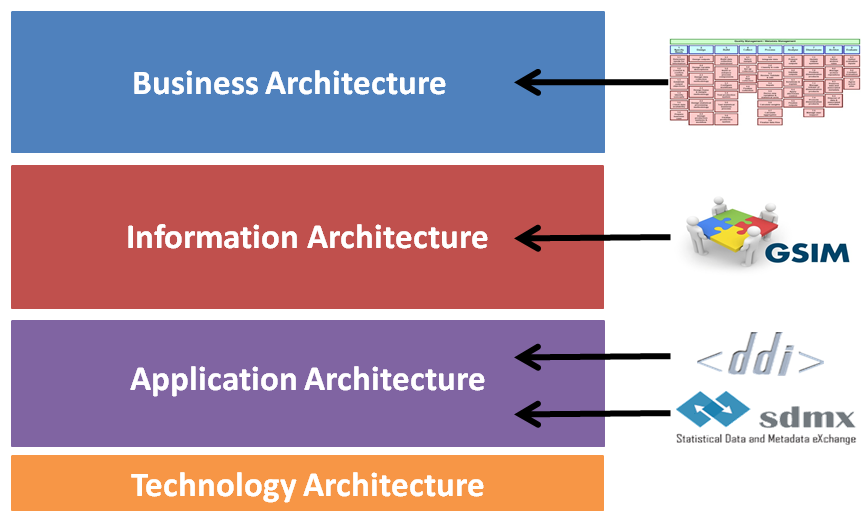
\includegraphics[height=5cm]{images/cspa-layer}
    \caption{Layer pada CSPA}
    \label{fig:cspa-layer}
\end{figure}

\section{Sistem Terdistribusi}
Salah satu mekanisme untuk menangani masalah pada pendekatan centralized adalah dengan menggunakan pendekatan sebaliknya, yakni dengan menggunakan sistem terdistribusi. Sistem terdistribusi dapat diartikan sebagai sebuah jaringan komputer untuk menyelesaikan masalah komputasi (\textit{computational problem}) dengan cara membagi \textit{task} ke dalam beberapa komputer (Godfrey, 2006)~\cite{_primer_????}. Setiap komputer dalam jaringan berkomunikasi dengan menggunakan metode \textit{message passing}~\cite{andrews_foundations_1999}. Keuntungan dari pemanfaatan sistem terdistribusi antara lain~\cite{takdir_multi-layer_2014}:
\begin{itemize}
\item Mempercepat \textit{response time} dan mengurangi \textit{traffic jaringan}, 
\item Meningkatkan kecepatan akses dan \textit{query} terhadap data, 
\item Meningkatkan system \textit{availability} dan menghindari kegagalan sistem dengan menerapkan \textit{single point of failure}.
\end{itemize}
Selain keuntungan, sistem terdistribusi juga memiliki beberapa tantangan, antara lain :
\begin{itemize}
\item Pembagian data (\textit{data partitioning}) dan proses komputasi (\textit{task}), 
\item Keselarasan data (\textit{data syncronization}).
\end{itemize}

\section{\textit{Grid Computing}}
\textit{Grid computing} dapat dianggap sebagai sebuah sistem terdistribusi yang bersifat \textit{non-interactive} antar \textit{node}. Masing-masing \textit{node} pada \textit{grid computers} menjalankan proses komputasi (\textit{task}) secara terpisah. Prinsip umum yang menjadi karakteristik \textit{grid}~\cite{baker_grids_2002}:
\begin{itemize}
\item Tersusun dari beberapa domain administrasi dan otonomi (\textit{geographically dispersed}), 
\item \textit{Heterogen} dan tersusun dari beragam teknologi yang bervariasi, 
\item \textit{Scalable}, dapat berkembang dari hanya beberapa \textit{integrated resources} menjadi ribuan bahkan jutaan, \textit{Dynamic} dan \textit{adaptable}, mampu mendeteksi \textit{resource failure} dan memanfaatkan \textit{available resource}.
\end{itemize}
Untuk mengakomodir \textit{heterogen resources}, maka \textit{grid} harus mengikuti prinsip berikut :
\begin{itemize}
\item Tidak menginterfensi domain administrasi dan otonomi yang sudah ada, 
\item Tidak perlu mengganti sistem operasi, protokol jaringan, atau \textit{services}, 
\item Memungkinkan \textit{remote sites} untuk bergabung atau meninggalkan jaringan kapanpun, 
\item Menyediakan sistem yang handal dan infrastruktur yang \textit{fault tolerance} dengan \textit{no single point of failure}, 
\item Menyediakan \textit{support} untuk komponen yang heterogen, 
\item Menggunakan teknologi yang telah ada dan terstandarisasi, 
\item Menyediakan sinkronisasi.
\end{itemize}

\section{\textit{Mobile Grid Computing}}
\textit{Mobile grid computing} dapat didefinisikan sebagai sebuah sistem terdistribusi berbasis \textit{grid computing} yang mengakomodir penggunaan \textit{mobile device}. \textit{Mobile device}, seperti \textit{PDA} dan \textit{smartphone}, biasanya diindikasikan dengan kekuatan pemrosesan yang lemah, kapasitas baterai yang terbatas, dan media penyimpanan yang terbatas. Menjalankan proses yang intensif pada \textit{mobile device} memerlukan kemampuan pemrosesan yang lebih, media penyimpanan, penyelesaikan proses dengan waktu seminimal mungkin, sehingga penggunaan \textit{mobile grid} dapat menjadi salah satu solusi~\cite{sathyan_job_2009}. \textit{Mobile grid computing} memungkinkan \text{mobility} dalam sebuah \textit{grid framework}, sehingga memungkinkan \textit{mobile device} dapat beroperasi secara halus (\textit{seamless}), transparan, aman dan efisien.

Zotll dkk telah meneliti sebuah metode untuk menyimpan informasi dalam tiga tingkatan (\textit{Three-tier}), (i) \textit{base tier}, (ii) \textit{information tier}, dan (iii) \textit{organization tier} yang dinamakan IRMA. Metode IRMA diterapkan pada \textit{mobile grid environment} dengan menggunakan \textit{Erasure Code}~\cite{zottl_three-tier_2008}. \textit{Erasure Code} (EC)~\cite{weatherspoon_erasure_2002} menggunakan skema \textit{replication} dan \textit{parity coding}. Skema replikasi bekerja dengan menduplikasi data pada beberapa \textit{node}, sementara skema \textit{parity coding} tidak menduplikasi data, tetapi menggunakan \textit{checksum} untuk me-\textit{recover} dari \textit{failure}. Pada \textit{mobile computing}, replikasi adalah cara yang umum digunakan untuk menjamin ketersediaan (\textit{persistency}). Beberapa strategi replikasi yang telah dikembangkan antara lain \textit{uniform}, \textit{proportional}, dan \textit{square-root}~\cite{lv_search_2002}. Replikasi dapat menjamin \textit{persistence} pada saat koneksi putus secara tiba-tiba (\textit{unpredicted disconnected}). Berdasarkan hasil penelitian, metode IRMA dapat bekerja secara konsisten, persisten, dan efisien dalam jaringan \textit{mobile grid} yang dinamis.

\section{\textit{Connectionless Grid Computing}}
Pada sistem terdistribusi berbasis \textit{mobile grid}, sebagian besar \textit{node} berupa \textit{mobile device}, seperti \textit{PDA} dan \textit{smartphone}. \textit{Mobile device} mempunyai karakteristik yang \textit{mobile}, dapat dengan mudah berpindah dari suatu lokasi ke lokasi yang lain. Lokasi dimana \textit{mobile device} ini berada terkadang merupakan lokasi yang tidak terjangkau oleh sinyal telekomunikasi atau \textit{wifi} area. Tidak terhubungnya suatu \textit{mobile node} dalam sebuah jaringan dapat dikelompokkan dalam beberapa jenis~\cite{gutwin_gone_2010}:
\begin{itemize}
\item \textit{Delay-based Interruption}, merupakan sebuah gap singkat (\textit{short-term gap}) dalam pengiriman pesan, 
\item \textit{Network Outage}, merupakan kondisi dimana sebuah \textit{mobile node} terputus dari jaringannya karena hilangnya jaringan komunikasi, 
\item \textit{Explicit Departures}, merupakan kondisi \textit{mobile node} keluar dari jaringan atau keluar dari aplikasi secara eksplisit
\end{itemize}
Ho dkk meneliti tentang penggunaan pendekatan \textit{connection-less} untuk mengakomodir permasalahan komunikasi~\cite{ho_connectionless_2004}. Pendekatan \textit{connection-less} ini bekerja secara \textit{ad-hoc} pada jaringan tanpa infrastruktur (\textit{infrastructure-less network}), sehingga memungkinkan \textit{mobile nodes} juga berperan sebagai \textit{router} yang mengakomodir komunikasi dengan \textit{mobile nodes} yang lain. Pendekatan \textit{connection-less} juga diteliti oleh Imran dkk~\cite{imran_proxy-based_2007} dengan menggunakan \textit{proxy-based checkpoint} dan \textit{message logging} yang dinamakan \textit{Mobile Host Proxies [MHP]}. Metode MHP menjadikan setiap \textit{mobile device} sebagai \textit{Mobile Host [MH]} dan \textit{Mobile Service Station [MSS]} dan menyimpan \textit{checkpoint} secara \textit{asyncronous}.

\section{Pola Implementasi SOA untuk Sistem Data-Intensif Terdistribusi}
Service Oriented Architecture (SOA) dapat dipandang dari dua perspektif yang berbeda : sebagai arsitektur bisnis (business architecture) dan arsitektur teknis (technical architecture). Dari sudut pandang bisnis, SOA menawarkan solusi dalam mengelola bisnis dengan menekankan pada layanan (services) sebagai unit/satuan terkecil yang perlu dirancang dan diorganisir. Sementara dari sudut pandang teknis, SOA memperkenalkan prinsip-prinsip dalam merancang dan mengembangkan perangkat lunak yang berorientasi service.

Service dalam konteks bisnis merupakan kumpulan aktifitas yang dijalankan oleh tiap-tiap unit kerja dalam suatu perusahaan. Dengan demikian, sebuah unit kerja dapat berperan sebagai penyedia layanan (service provider) bagi unit kerja lain yang membutuhkan (service consumer), dan sebaliknya. Hubungan antar penyedia dan pengguna layanan diatur dalam sebuah perjanjian (contract), yang berisi penjelasan dari layanan serta syarat dan ketentuan yang harus dipenuhi kedua belah pihak.

Service dalam konteks teknis, mengadopsi konsep service yang diterapkan dalam konteks bisnis. Akan tetapi, service dalam konteks teknis diinterpretasikan dalam fungsi-fungsi yang didukung oleh software, atau dikenal dengan logika bisnis (business logic). Logic business dikemas dalam bentuk komponen software dengan mekanisme tertentu sehingga dapat didistribusikan.

Thomas Erl memperkenalkan prinsip-prinsip dalam merancang software service, yang bertujuan utnuk memudahkan integrasi sistem informasi, yaitu:
\begin{itemize}
\item Standardize Service Contract

Services yang terdapat pada sistem inventarisasi yang sama memiliki desain kontrak yang serupa.
\item Service Loose Coupling

Service tidak memiliki ketergantungan terhadap lingkungan atau platform tertentu.
\item Service Abstraction

Service provider hanya menyediakan informasi dasar, sementara teknis implementasi service tidak disertakan dalam kontrak.
\item Service Reusability

Service tidak dirancang untuk keperluan tunggal, tetapi bersifat multi-purpose. Sebuah service merupakan enterprise resource yang dapat digunakan kembali.
\item Service Statelessness

Meminimalisir penggunaan resources dengan tidak menyertakan pengelolaan state pada service.
\item Service Discoverability

Service dilengkapi dengan metadata, sehingga dapat ditelusuri secara efektif.
\item Service Composability

Sebuah service dapat tersusun dari penggabungan beberapa service.
\end{itemize}

SOA hanyalah merupakan sebuah arsitektur, sehingga diperlukan teknologi pendukung agar dapat direalisasikan. Web service merupakan salah satu teknologi yang dapat digunakan untuk merealisasikan konsep SOA menjadi sebuah sistem software. Web service menggunakan teknologi XML yang didesain sedemikian rupa sehingga mendukung komunikasi antar komponen software yang bersifat platform independent (W3C 2004).

XML sendiri merupakan dokumen teks yang mengikuti format dan spesifikasi tertentu sehingga mudah untuk diproses oleh mesin/komputer. Tujuan yang ingin dicapat dari XML (W3C 2006) antara lain :
\begin{itemize}
\item XML harus dapat digunakan pada jaringan Internet,
\item XML harus dapat diaplikasikan secara luas,
\item Adanya kemudahan pembuatan program (software) untuk memproses dokumen XML,
\item Meminimalkan jumlah fitur yang tidak harus ada,
\item Dokumen XML harus dapat terbaca dengan layak oleh manusia,
\item Dokumen XML harus mudah dibuat.
\end{itemize}

Teknologi Web service mengadopsi XML dalam format Web Service Definition Language (WSDL). WSDL menyediakan informasi kepada service consumer berupa struktur data yang diperlukan, jenis operasi yang didukung, data binding, protokol komunikasi data, maupun endpoint. SOAP merupakan protokol komunikasi yang ditujukan untuk menangani pertukaran data antara service provider dan service consumer. Selain mendefinisikan struktur data, SOAP juga menyertakan nilai dari setiap atribut.

Pada penelitiannya, Takdir dkk telah mencoba menemukan pola implementasi SOA pada aplikasi yang bersifat data intensif. Aplikasi data intensif memiliki ciri : (i) tersusun dari sederetan operasi yang mengolah data dalam jumlah besar, dan (ii) adanya aliran data dengan volume yang besar antar operasi-operasi tersebut (Habich, Richly, Preissler, et al. 2008). Pola implementasi SOA rancangan Takdir dkk bertujuan untuk menjembatani gap antara desain business services dan software service. Proses perancangan pola implementasi menitikberatkan pada layanan statistik (statistical services) yang bersifat data intensif.

Perancangan pola implementasi dibagi menjadi dua, implementasi logik workflow dan implementasi web services. Mekanisme eksekusi logik workflow dan web services, sebagaimana dalam Gambar \ref{fig:design-workflow-webservice}, dalam pengujian dibagi dalam 4 (empat) skenario :
\begin{enumerate}
\item Pengeksekusian workflow dan web services dilakukan pada infrastruktur pusat,
\item Pengeksekusian workflow dilakukan pada infrastruktur lokal, sementara pengeksekusian web service dilakukan pada infrastruktur pusat,
\item Pengeksekusian workflow dilakukan pada infrastruktur pusat, dan web service pada infrastruktur lokal,
\item Pengeksekusian workflow dan web services dilakukan pada infrastruktur lokal.
\end{enumerate}
Instilah infrastruktur pusat disini merujuk pada infrastruktur TIK yang ada di BPS Pusat, sementara istilah infrastruktur lokal merujuk pada infrastruktur TIK pada BPS Daerah.

\begin{figure}[H]
    \begin{subfigure}{.5\textwidth}
  		\centering
  		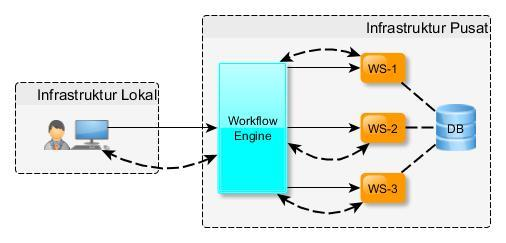
\includegraphics[width=.8\linewidth]{images/design-1}
  		\caption{Skenario 1}
  		\label{fig:design-workflow-webservice-1}
	\end{subfigure}%
	\begin{subfigure}{.5\textwidth}
  		\centering
  		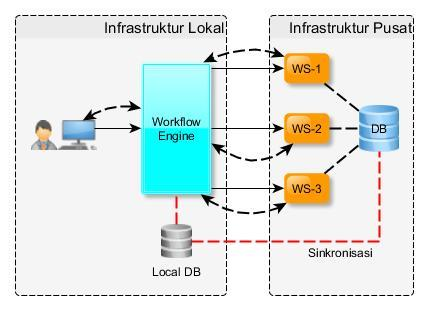
\includegraphics[width=.8\linewidth]{images/design-2}
  		\caption{Skenario 2}
  		\label{fig:design-workflow-webservice-2}
	\end{subfigure}
	\begin{subfigure}{.5\textwidth}
  		\centering
  		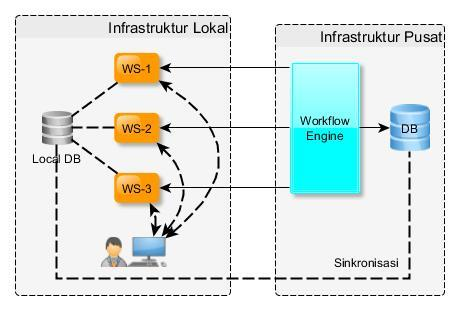
\includegraphics[width=.8\linewidth]{images/design-3}
  		\caption{Skenario 3}
  		\label{fig:design-workflow-webservice-3}
	\end{subfigure}%
	\begin{subfigure}{.5\textwidth}
  		\centering
  		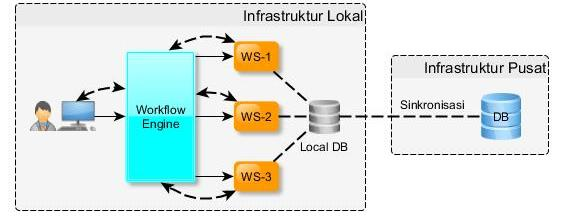
\includegraphics[width=.8\linewidth]{images/design-4}
  		\caption{Skenario 4}
  		\label{fig:design-workflow-webservice-4}
	\end{subfigure}
    \caption{Skenario Eksekusi Logik Workflow dan Web Services}
    \label{fig:design-workflow-webservice}
\end{figure}

Pada skenario yang melibatkan infrastruktur pusat dan infrastruktur lokal, terdapat mekanisme sinkronisasi pada database. Selain itu, pada skenario yang menempatkan web services pada repository lokal juga diperlukan sinkronisasi web services, antara central repository dan local repository. Proses sinkronisasi, baik database maupun web services, antara infrastruktur pusat dan infrastruktur lokal dilakukan untuk menjaga konsistensi antara keduanya.

\begin{figure}[H]
    \centering
    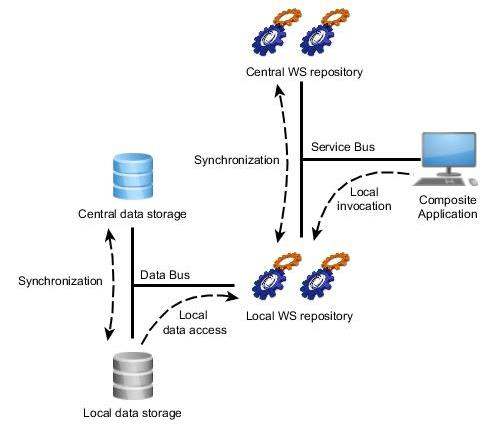
\includegraphics[height=5cm]{images/syncronize}
    \caption{Sinkronisasi Data dan Web Service}
    \label{fig:syncronize}
\end{figure}

Selain mekanisme sinkronisasi, pada skenario yang melibatkan infrastruktur pusat dan daerah juga terdapat mekanisme replikasi. Replikasi, baik database maupun web services dilakukan dengan menggunakan pendekatan cache. Tujuan replikasi adalah untuk mendekatkan data maupun web service kepada service consumer. Replikasi data sangat tergantung pada replikasi web service, karena hanya data yang dibutuhkan oleh web service yang akan direplika.

\begin{figure}[H]
    \centering
    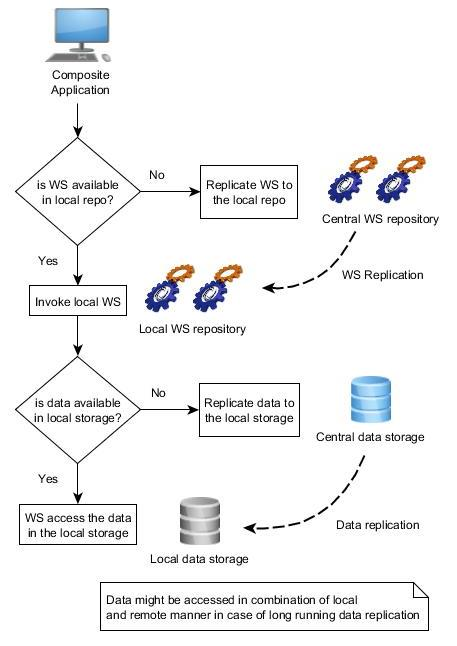
\includegraphics[height=5cm]{images/replication}
    \caption{Proses Replikasi Data dan Web Service}
    \label{fig:replication}
\end{figure}

Terdapat beberapa skenario deployment yang mengakomodir empat pendekatan eksekusi logik dan web service :
\begin{enumerate}
\item Web service dan data terpusat

Pada skenario ini, web services (task-centric web service dan data service) dan database dipusatkan pada server seperti pada Gambar \ref{fig:deployment-1} Skenario ini cocok untuk web service yang membutuhkan akses terhadap data yang bersifat global dan memiliki parameter dengan ukuran data yang kecil.

\begin{figure}[H]
    \centering
    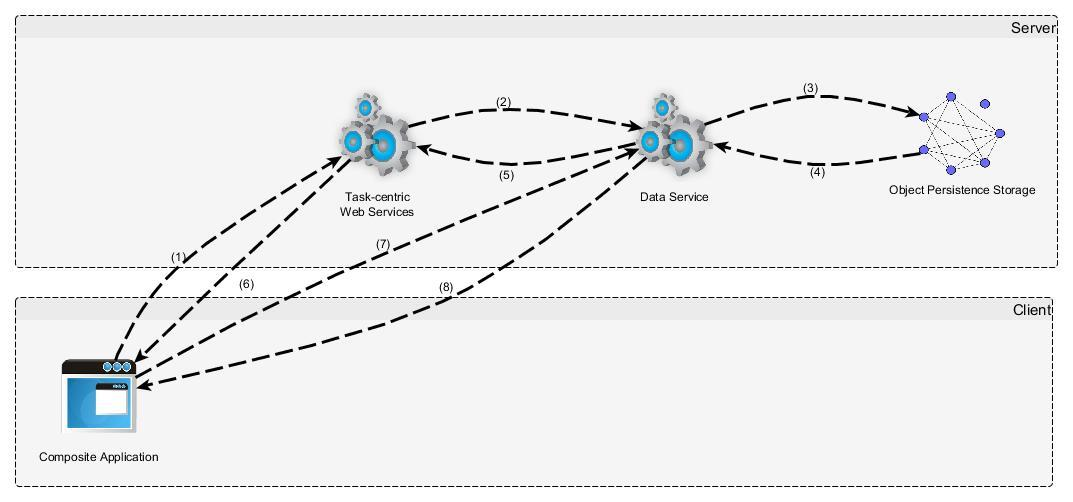
\includegraphics[height=5cm]{images/deployment-1}
    \caption{Skenario Deployment Web Service dan Data Terpusat}
    \label{fig:deployment-1}
\end{figure}

\item Web service terdistribusi, data terpusat

Logik task-centric web services direplika ke client untuk dieksekusi. Logik direpresentasikan dalam bentuk file *.class untuk kemudian di-load ke runtime dengan Java Reflection API . Setelah file yang berisi logik direplika, maka client akan menjalankan servlet engine pada Apache CXF untuk melakukan hosting web service. Dalam hal ini, client juga berperan sebagai server (service provider) bagi dirinya sendiri, maupun client lain yang terkoneksi dengannya.

\begin{figure}[H]
    \centering
    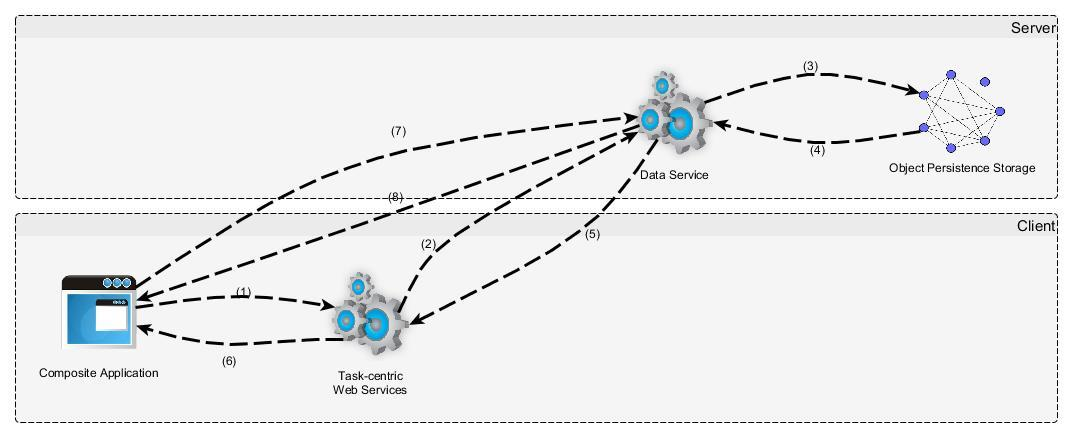
\includegraphics[height=5cm]{images/deployment-2}
    \caption{Skenario Deployment Web Service Terdistribusi, Data Terpusat}
    \label{fig:deployment-2}
\end{figure}

\item Web service dan data terdistribusi

Skenario ini ditujukan untuk memungkinkan sistem bekerja secara offline (disconnected) dimana semua komponen software yang dibutuhkan oleh client direplikasi, baik data, maupun web services. Komunikasi antarkomponen berjalan pada infrastruktur lokal, kecuali proses sinkronisasi data dengan server yang dilakukan secara asynchronous. DataObjek yang direplika ke object persistence datastore pada client adalah DataObject yang hanya dibutuhkan oleh task-centric web sevices yang telah direplika pada client. Setelah replikasi berlangsung, maka infrastruktur lokal dapat beroperasi meskipun kehilangan koneksi dengan infrastruktur pusat. Proses sinkronisasi data dapat dilakukan secara asynchronous ketika koneksi ke infrastruktur pusat tersedia kembali. Gambar \ref{fig:deployment-3a} merupakan gambaran skenario tersebut.

\begin{figure}[H]
    \centering
    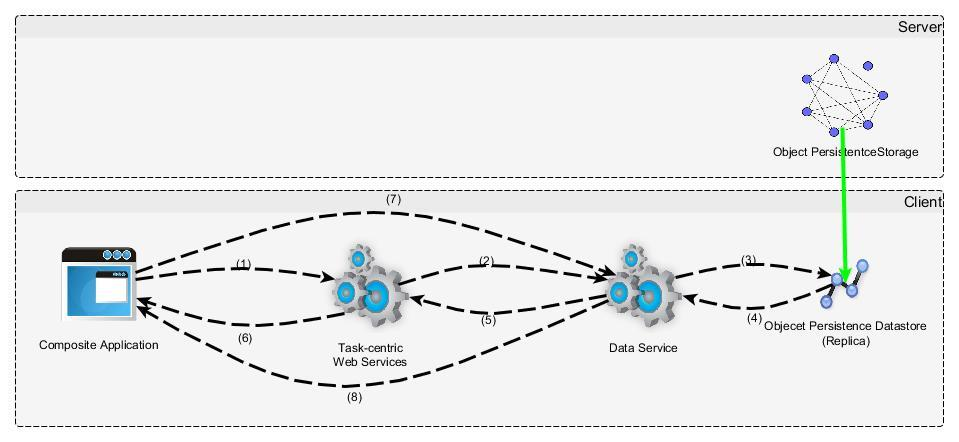
\includegraphics[height=5cm]{images/deployment-3a}
    \caption{Skenario Deployment Web Service dan Data Terdistribusi}
    \label{fig:deployment-3a}
\end{figure}

Pada saat replikasi data dari infrastruktur pusat ke infrastruktur lokal sedang berlangsung, teknologi In-Memory Data Grids (IMDG) digunakan agar operasi di client dapat tetap berjalan sementara proses replikasi berjalan secara asynchronous. Hal ini juga berlaku untuk proses sinkronisasi data dari infrastruktur lokal ke infrastruktur pusat, maupun sebaliknya.

\begin{figure}[H]
    \centering
    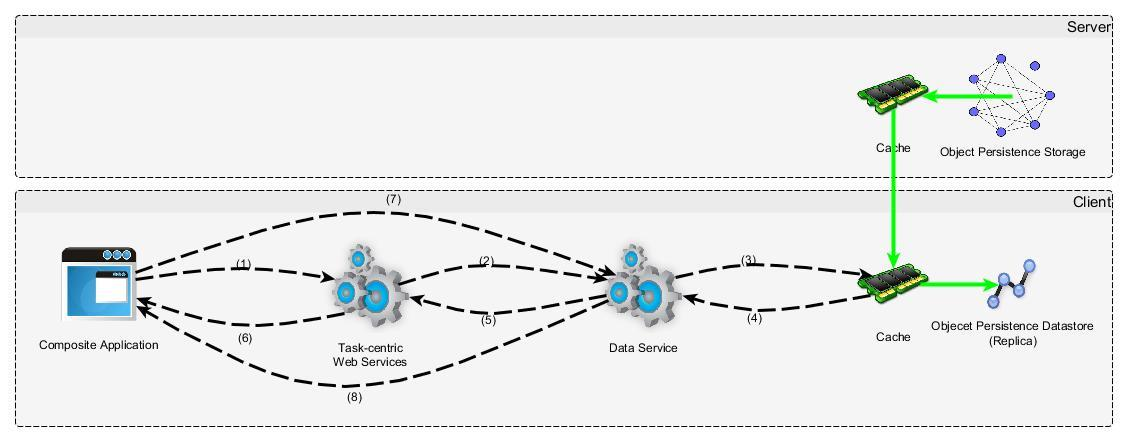
\includegraphics[height=5cm]{images/deployment-3b}
    \caption{Proses Replikasi Data dengan IMDG}
    \label{fig:deployment-3b}
\end{figure}
\end{enumerate}

Pada tahap pengujian, data yang digunakan adalah data Kor SUSENAS 2009, yang terdiri dari 129 fields. Adapun variabel yang diamati dalam mengevaluasi kinerja sistem adalah : 1) Response Time, 2) Network utilization, dan 3) CPU utilization. Pengujian yang dilakukan pada environment virtual machine, dengan konfigurasi yang telah disesuaikan dengan kondisi yang sebenarnya, diperoleh hasil sebagai berikut :
\begin{enumerate}
\item Skenario web service dan data terpusat

\begin{table}[H]
\begin{minipage}{\linewidth}
\centering
\begin{tabular}{|l|l|l|}
\hline
%\rowcolor[HTML]{C0C0C0} 
\textbf{Jumlah Records} & \textbf{Fully Centralized} & \textbf{Distributed} \\ \hline
5           & 00:00:04.627            & 00:00:02.484                  \\ \hline
10           & 00:00:08.320            & 00:00:03.205                  \\ \hline
100           & 00:02:00.142         & 00:00:12.648                  \\ \hline
200           & 00:04:01.497             & 00:00:22.653                 \\ \hline
500           & 00:10:02.997             & 00:01:50.549                 \\ \hline
\end{tabular}
\caption{Response Time Pengujian Skenario I}
\label{table:testing-1-response-time}
\end{minipage}
\end{table}

\begin{table}[H]
\begin{minipage}{\linewidth}
\centering
\begin{tabular}{|l|l|l|}
\hline
%\rowcolor[HTML]{C0C0C0} 
\textbf{Jumlah Records} & \textbf{Fully Centralized} & \textbf{Distributed} \\ \hline
5           & 748            & 7.64                  \\ \hline
10           & 1382.4            & 7.53                  \\ \hline
100           & 20449.28         & 7.76                  \\ \hline
200           & 40908.8             & 7.64                 \\ \hline
500           & 102256.64             & 7.64                 \\ \hline
\end{tabular}
\caption{Total Traffic Size Pengujian Skenario I}
\label{table:testing-1-traffic}
\end{minipage}
\end{table}

\item Skenario web service terdistribusi, data terpusat

\begin{table}[H]
\begin{minipage}{\linewidth}
\centering
\begin{tabular}{|l|l|l|}
\hline
%\rowcolor[HTML]{C0C0C0} 
\textbf{Jumlah Records} & \textbf{Fully Centralized} & \textbf{Distributed} \\ \hline
5           & 00:00:14.470            & 00:00:09.530                  \\ \hline
10           & 00:00:14.872            & 00:00:10.745                  \\ \hline
100           & 00:01:15.759         & 00:00:23.183                  \\ \hline
200           & 00:02:22.225             & 00:00:37.554                 \\ \hline
500           & 00:05:39.980             & 00:02:43.895                 \\ \hline
\end{tabular}
\caption{Response Time Pengujian Skenario II}
\label{table:testing-2-response-time}
\end{minipage}
\end{table}

\begin{table}[H]
\begin{minipage}{\linewidth}
\centering
\begin{tabular}{|l|l|l|}
\hline
%\rowcolor[HTML]{C0C0C0} 
\textbf{Jumlah Records} & \textbf{Fully Centralized} & \textbf{Distributed} \\ \hline
5           & 365.62            & 449.88                  \\ \hline
10           & 692.19            & 934.07                  \\ \hline
100           & 10240         & 12400.64                  \\ \hline
200           & 20490.24             & 27084.8                 \\ \hline
500           & 51210.24             & 38840.32                 \\ \hline
\end{tabular}
\caption{Total Traffic Size Pengujian Skenario II}
\label{table:testing-2-traffic}
\end{minipage}
\end{table}

\item Skenario web service dan data terdistribusi

\begin{enumerate}
\item Response Time

Waktu yang dibutuhkan untuk melakukan updating web service (error correction service) adalah 00:00:04,647.
\item Network Utilization

Total taffic yang dihasilkan sebesar 17.21 kilobytes. Ukuran tersebut merupakan file logik web service yang di-download oleh client.

\begin{figure}[H]
    \centering
    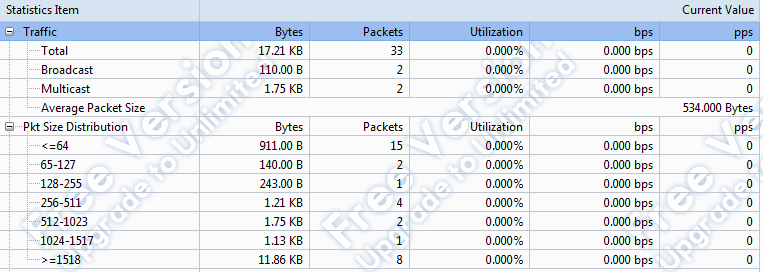
\includegraphics[height=5cm]{images/testing-3-network}
    \caption{Network Utilization Proses Patching/Updating Web Service}
    \label{fig:testing-3-network}
\end{figure}

\item CPU Utilization

Processor time yang dihasilkan mesin client pada Gambar \ref{fig:testing-3-cpu} merupakan proses untuk melakukan hosting web service yang di-download dari server. Proses tersebut menggunakan sekitar 50 persen processor time dari masing-masing CPU core.

\begin{figure}[H]
    \centering
    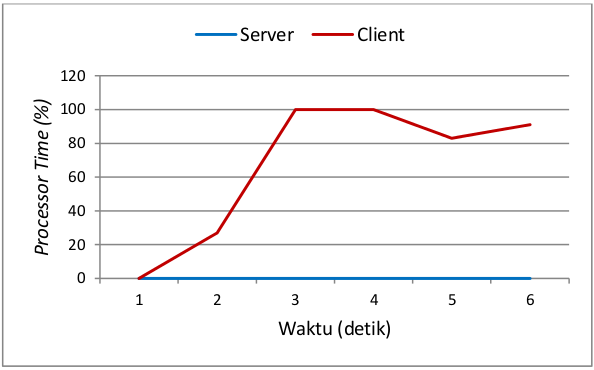
\includegraphics[height=5cm]{images/testing-3-cpu}
    \caption{Grafik CPU Utilization Proses Updating Web Service}
    \label{fig:testing-3-cpu}
\end{figure}
\end{enumerate}
\end{enumerate}
